\subsection{Alfabeti e parole}
\begin{defi}[Insieme delle parole su un alfabeto]
    Fissato un alfabeto $A$, si definisce \textit{l'insieme delle parole definite su $A$} come l'insieme
\[
A^* := \bigcup_{k \geq 0} A^{\{1,\dots,k\}}.
\]
dove $A^{\{1,\dots,k\}}:=\{ f \text{ è una funzione}\, | \, f: \{ 1, \dots ,k\} \to A\}$.
\end{defi}
Si noti che per convenzione l'insieme $\{1, \dots, k\}$ per $k = 0$ corrisponde all'insieme vuoto. E pertanto l'insieme $A^*$ per definizione contiene anche la funzione $A^{\emptyset}$ che è detta la \textit{parola vuota}.

\begin{defi}[Lunghezza di una parola]
Si può definire la funzione ``lunghezza'' di una parola $|u|$ come il più piccolo $n$ tale che $u \in A^{\{1,\dots,n\}}$.
\end{defi}

\begin{defi}[Concatenazione di parole]
La concatenazione di due parole $u$ e $v$ sarà una funzione $uv \in A^{\{1,\dots,|u|+|v|\}}$ tale che
\[
uv(k) = \begin{cases} u(k) & \text{se } k \leq |u| \\ v(k - |u|) & \text{se } |u|+1 \leq k \leq |u|+|v| \end{cases}
\]
\end{defi}
\begin{rema}
Equivalentemente, possiamo introdurre  l'insieme delle parole su $A$, con $A^*$, come l'insieme delle successioni finite di elementi di $A$ (compresa la parola vuota). Se $u, v \in A^*$ allora $uv \in A^*$ indicherà la parola ottenuta concatenando $u$ con $v$. 
\end{rema}
\subsection{Algoritmo}
\begin{defi}[Algoritmo]
    Un \textit{algoritmo} è una sestupla $\mathcal A:=(A,B,C,\epsilon, \tau, \delta)$ dove
    $A$ e $B$ sono insiemi chiamati rispettivamente \textit{alfabeto di entrata} e \textit{alfabeto di uscita}, $C$ è un insieme chiamato \textit{spazio di configurazioni possibili} e tre funzioni
\begin{align*} \epsilon &: A^* \to C \\ \tau &: C \to C \\ \delta &: C \to B^* \end{align*}
La \textit{computazione associata ad una parola} $w \in A^*$ è la successione
\[
(\epsilon(w), \tau(\epsilon(w)), \tau^2(\epsilon(w)), \dots)
\]
diremo che questultima è \textit{finita} (oppure diremo che \textit{termina}) se esiste un $n \in \mathbb N$ tale che $\tau ^n(\epsilon(w))\in dom(\delta)$, altrimenti diremo che è \textit{infinita}.
Se la  sequenza termina in una configurazione $\tau^n(\epsilon(w))$ allora avremo che il \textit{risultato della computazione} è $\delta(\tau^n(\epsilon(w)))$.
Se invece la computazione associata non termina si dirà che l'algoritmo \textit{non termina partendo da $w$}.
\end{defi}
\begin{center}
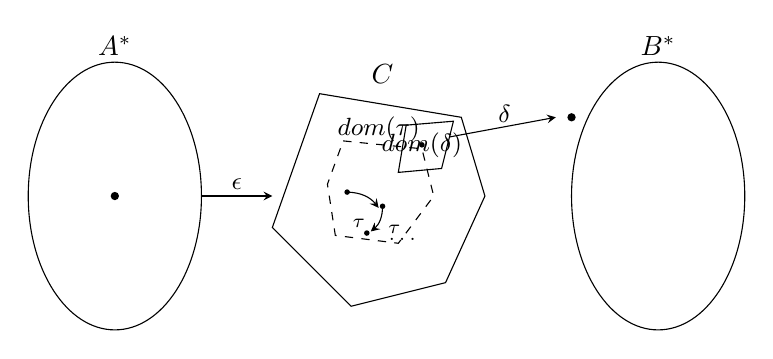
\begin{tikzpicture}[>=stealth, scale=1]

% A*
\draw (0,0) ellipse (1.1cm and 1.7cm);
\node at (0,1.9) {$A^*$};
\fill (0,0) circle (1.5pt);

% C (poligono irregolare)
\draw (2.6,1.3) -- (4.4,1.0) -- (4.7,0) -- (4.2,-1.1) -- (3.0,-1.4) -- (2.0,-0.4) -- cycle;
\node at (3.4,1.55) {$C$};

% dom(tau), regione tratteggiata dentro C
\draw[dashed] (2.9,0.7) -- (3.9,0.6) -- (4.05,0) -- (3.6,-0.6) -- (2.8,-0.5) -- (2.7,0.15) -- cycle;
\node[font=\small] at (3.35,0.85) {$dom(\tau)$};

% punti e frecce tau (successione di transizioni)
\fill (2.95,0.05) circle (1pt);
\draw[->] (2.95,0.05) to[bend left=25] (3.35,-0.15);
\node[font=\scriptsize] at (3.1,-0.35) {$\tau$};

\fill (3.4,-0.13) circle (1pt);
\draw[->] (3.4,-0.13) to[bend left=25] (3.25,-0.45);
\node[font=\scriptsize] at (3.55,-0.42) {$\tau$};

\fill (3.2,-0.47) circle (1pt);
\node[font=\scriptsize] at (3.65,-0.55) {$\ldots$};

% dom(delta)
\draw (3.7,0.9) -- (4.3,0.95) -- (4.15,0.35) -- (3.6,0.3) -- cycle;
\node[font=\small] at (3.9,0.65) {$dom(\delta)$};
\fill (3.9,0.65) circle (1pt);

% freccia epsilon: A* -> C
\draw[->] (1.1,0) -- (2.0,0);
\node[font=\small] at (1.55,0.15) {$\epsilon$};

% freccia delta: dom(delta) -> B*
\draw[->] (4.25,0.75) -- (5.6,1.0);
\node[font=\small] at (4.95,1.05) {$\delta$};
\fill (5.8,1.0) circle (1.5pt);

% B*
\draw (6.9,0) ellipse (1.1cm and 1.7cm);
\node at (6.9,1.9) {$B^*$};

\end{tikzpicture}
\end{center}

\footnotetext{Tesi di Church: l'insieme dei risultati di equivalenza tra vari modelli effettivi di calcolo è noto come Tesi di Church, che afferma che tutti i modelli di calcolo si equivalgono.}

\begin{defi}[Funzione associata ad un algoritmo]Sia $\mathcal A:=(A,B,C,\epsilon, \tau, \delta)$ un algoritmo. Possiamo definire la funzione
\[
\begin{matrix}
f_\mathcal{A} : & A^* & \to & B^*
\\
& w & \mapsto &  \begin{cases} \delta(\tau^n(\epsilon(w))) & \text{se } n \text{ è il più piccolo intero}
\\ & \text{per cui } \tau^n(\epsilon(w)) \in dom(\delta) \text{ ,} 
\\ \bot & \text{se } \mathcal A \text{ non termina partendo da } w \end{cases}
\end{matrix}
\]
che chiameremo \textit{funzione associata all'algoritmo} $\mathcal A$.
\end{defi}

In pratica, ogni volta che diremo che la funzione $f$ associata ad un certo algoritmo formale è definita per ogni possibile parola $w \in A^*$, intenderemo dire che per ogni possibile input la computazione termina e restituisce attraverso la funzione di output $\delta$ il valore della funzione $f(w)$.

\begin{defi}[Funzione caratteristica]
La funzione $\mathbf{1}_X$ è la \textit{funzione caratteristica} (o indicatrice) dell'insieme $X$, definita come
\[
\mathbf{1}_X(w) = \begin{cases} 1 & w \in X \\ 0 & w \notin X. \end{cases}
\]
\end{defi}

\begin{defi}[Algoritmo che decide un insieme]
Diremo che un certo \textit{algoritmo decide} un insieme $X \subset A^*$ quando la funzione associata all'algoritmo coincide con la funzione caratteristica di $X$, quindi se vale:
\[
f_\mathcal{A}(x) = \mathbf{1}_X(x) \text{ per ogni } x \in A^*.
\]
\end{defi}
\begin{defi}[Algoritmo che semidecide un insieme]
Diremo che un certo algoritmo  \textit{semidecide} un insieme
$X \subseteq A^*$ quando la funzione parziale associata all'algoritmo
$f_{\mathcal A}$ è definita esattamente sugli elementi di $X$ e, quando è
definita, restituisce il valore $1$. In altre parole:
\[
f_{\mathcal A}(x)=
\begin{cases}
1, & \text{se } x\in X,\\
\bot, & \text{se } x\notin X,
\end{cases}
\]
dove il simbolo $\bot$ indica che l'algoritmo non termina.
\end{defi}

\begin{rema}
Questa è chiaramente una funzione totale pertanto nella definizione, implicitamente, stiamo affermando che quando un algoritmo decide un insieme, la computazione dell'algoritmo a partire da una qualsiasi parola di alfabeto $A$ termina.
\end{rema}
\textcolor{red}{controlla qui:}
Pertanto, consideriamo i processi computazionali come metodi di decisione simbolici, in cui si rende automatico (per questo formalmente ineccepibile) il metodo di decisione di una proprietà. Le garanzie sulla correttezza della decisione vengono dalla verificabilità: il processo lavora su sequenze di simboli, e applica in maniera asettica alcune regole di trasformazione (i principi deduttivi) in maniera puntuale: da cui viene la richiesta specifica che le regole di trasformazione siano locali, applicabili in tempo finito e soprattutto in modo che la verifica della corretta applicazione sia finita.

In questo quadro, se anche il problema di decisione riguardasse un insieme di cardinalità più che numerabile, un processo computazionale finito potrebbe procedere modificando ed essendo influenzato solo da un numero finito di elementi. Quindi è la descrizione stessa del problema che ha senso solo quando è finita.

Con queste premesse la classe dei problemi più semplici che si possono porre è in prima istanza quella dei \textit{problemi di decisione} per un fissato alfabeto $A = \{a_1, \dots, a_n\}$. Essi consistono nella possibilità di definire un metodo per stabilire la separazione tra le parole di un sottoinsieme $X \subset A^*$ e quelle del complemento $A^* \setminus X$, procedura con le caratteristiche che abbiamo ricordato.